\documentclass{beamer}
\usepackage{caption}
\usepackage{float}
\usepackage{lscape}
\usepackage{graphicx}% http://ctan.org/pkg/graphicx
\usepackage{booktabs}% http://ctan.org/pkg/booktabs
\usepackage{array}
\usepackage[export]{adjustbox}
\usepackage{amsmath}
\usepackage{amsfonts}
\usepackage{amssymb}
\usepackage{tikz}
\usepackage{ upgreek }
\usepackage{subcaption}

% version as of 10.26 2/24/19

\graphicspath{ {images/} }
\usetheme{Madrid}
\definecolor{Gold}{RGB}{218,165,32}
\setbeamertemplate{navigation symbols}{}
\setbeamertemplate{theorems}[numbered]
\setbeamertemplate{theorems}[ams style] 
\renewcommand{\qedsymbol}{$\blacksquare$}

\makeatletter

\setbeamerfont{footline}{size=\fontsize{6.5}{8.5}\selectfont}

\defbeamertemplate*{footline}{Dan P theme}
{
  \leavevmode%
  \hbox{%
  \begin{beamercolorbox}[wd=.15\paperwidth,ht=2.25ex,dp=1ex,center]{author in head/foot}%
    \usebeamerfont{author in head/foot}\insertshortauthor\expandafter\beamer@ifempty\expandafter{\beamer@shortinstitute}{}{~~(\insertshortinstitute)}
  \end{beamercolorbox}%
  \begin{beamercolorbox}[wd=.62\paperwidth,ht=2.25ex,dp=1ex,center]{title in head/foot}%
    \usebeamerfont{title in head/foot}\insertshorttitle
  \end{beamercolorbox}%
  \begin{beamercolorbox}[wd=.23\paperwidth,ht=2.25ex,dp=1ex,right]{date in head/foot}%
    \usebeamerfont{date in head/foot}\insertshortdate{}\hspace*{1.5em}
\insertframenumber{} / \inserttotalframenumber\hspace*{4ex} 
  \end{beamercolorbox}}%
  \vskip0pt%
}
\makeatother

\title{Cross-Industry Dispersion and Expected Returns \\ (Pinchuk 2019)}

% A subtitle is optional and this may be deleted
%\subtitle{Optional Subtitle}

\author{Mykola Pinchuk}

\date{08/19/2019}

\subject{Empirical Asset Pricing}

\AtBeginSubsection[]

\begin{document}

\begin{frame}
  \titlepage
\end{frame}


\begin{frame}{Introduction}
\begin{itemize}
    \item {Cross-Industry Dispersion (CID) measures dispersion of returns across industries at a given point in time.}
    \item {High CID may reflect economic uncertainty.}
    \item {Is it a state variable from ICAPM?}
\end{itemize}
\end{frame}


\begin{frame}{Economic driving forces}\\
{High CID implies:}
\vspace{1cm}
\begin{itemize}
    \item {Structural changes in economy and increased economic uncertainty. $\mathbb{E}_t[\sigma(Income_{t+1})]\uparrow$.}
    \item {Some industries are struggling. Labor income risk increases, assuming that employees can not easily switch industries. In reality, labor income risk is rarely hedged.}
    \item {Additionally, it proxies for idiosyncratic risk.}
\end{itemize}
\end{frame}


\begin{frame}{Diversification assumptions and 4 channels}
\begin{enumerate}
    \item {Everybody can invest in market and hedge labor income. \\
    CID works, if it predicts future market returns (mean or sd). This is probably structural risk (ch.1).}
    \item {Everybody can invest in market, but not hedge labor income. \\
    CID works via ch.1 or ch.2 (labor income risk).}
    \item {Many people invest in industries (e.g., industry mutual funds, venture capital funds). \\
    CID works via ch.1, 2 or ch.3 (industry stock market risk).}
    \item {Many people invest in separate stocks. \\
    CID works via ch.1, 2, 3 or ch.4 (pure idiosyncratic risk).}
\end{enumerate}
\end{frame}


\begin{frame}{Cross-Industry Dispersion}
\begin{itemize}
    \item {Cross-Industry Dispersion (CID) is a mean absolute deviation of the returns of FF49 industries.}
    \item {CID is measured at daily frequency.}
    $$CID_t = [\frac{1}{N}\sum^{N}_{i=1}{|R_i-R_{MKT}|}]_t$$
    \item {I calculate sensitivity of stocks to CID and expect negative price of risk.}
\end{itemize}
\end{frame}


\begin{frame}{Cross-Industry Dispersion}
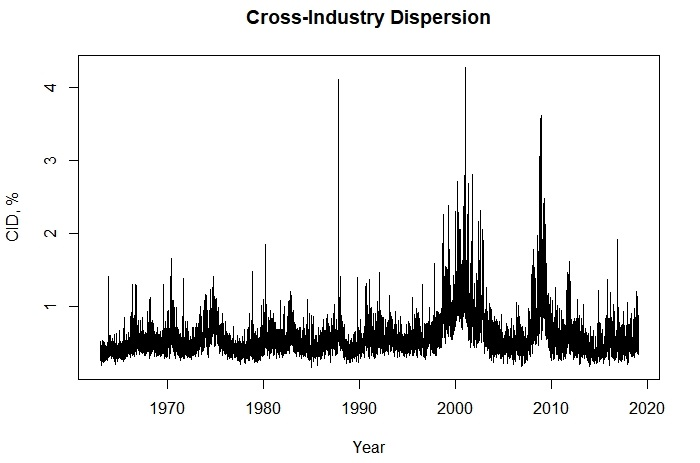
\includegraphics[width=1\textwidth]{ts_cid_00.jpeg}
\end{frame}


\begin{frame}{Sensitivity to Cross-Industry Dispersion}
\begin{itemize}
    \item {The sample covers 1963-2018.}
    \item {I estimate betas of stocks with respect to CID every day using 1 year of daily data.}
    \item {At the beginning of every month, stocks are divided into decile portfolios on their $\beta_{CID}$.}
    \item {I expect that low $\beta_{CID}$ stocks are risky and generate higher returns.}
    
\end{itemize}

\end{frame}



\begin{frame}{Return spread}

% Table created by stargazer v.5.2.2 by Marek Hlavac, Harvard University. E-mail: hlavac at fas.harvard.edu
% Date and time: Sun, Aug 18, 2019 - 5:05:42 PM
\begin{table}[!htbp] \centering 
  \caption{Excess returns of decile $\beta_{CID}$-sorted portfolios} 
  \label{} 
  \scriptsize
\begin{tabular}{@{\extracolsep{-6pt}} cccccccccccc} 
\\[-1.8ex]\hline 
\hline \\[-1.8ex] 
 & D1 & D2 & D3 & D4 & D5 & D6 & D7 & D8 & D9 & D10 & LS(annualized) \\ 
\hline \\[-1.8ex] 
Mean ew & $0.069$ & $0.052$ & $0.047$ & $0.047$ & $0.044$ & $0.043$ & $0.045$ & $0.042$ & $0.039$ & $0.034$ & $$-$8.828$ \\ 
T\_stat & $7.800$ & $7.044$ & $6.682$ & $6.682$ & $6.221$ & $5.774$ & $5.810$ & $5.133$ & $4.345$ & $3.172$ & $$-$5.021$ \\ 
Mean vw & $0.037$ & $0.027$ & $0.031$ & $0.030$ & $0.026$ & $0.029$ & $0.029$ & $0.022$ & $0.019$ & $0.009$ & $$-$7.215$ \\ 
T\_stat & $3.391$ & $2.949$ & $3.624$ & $3.685$ & $3.253$ & $3.532$ & $3.438$ & $2.428$ & $1.894$ & $0.669$ & $$-$2.733$ \\ 
\hline \\[-1.8ex] 
\end{tabular} 
\end{table}

% Table created by stargazer v.5.2.2 by Marek Hlavac, Harvard University. E-mail: hlavac at fas.harvard.edu
% Date and time: Sun, Aug 18, 2019 - 5:07:25 PM
\begin{table}[!htbp] \centering 
  \caption{Abnormal returns of value-weighted long/short portfolios} 
  \label{} 
\begin{tabular}{@{\extracolsep{5pt}} ccccc} 
\\[-1.8ex]\hline 
\hline \\[-1.8ex] 
Statistic & Ret & Alpha CAPM & Alpha FF3 & Alpha FF5 \\ 
\hline \\[-1.8ex] 
Return & -7.308 & -8.316 & -11.088 & -10.332 \\ 
T-stat & [ -2.730] & [ -3.216] & [ -4.516] & [ -4.165] \\ 
\hline \\[-1.8ex] 
\end{tabular} 
\end{table}
\end{frame}


\begin{frame}{Loadings}

\vspace{-0.64cm}

% Table created by stargazer v.5.2.2 by Marek Hlavac, Harvard University. E-mail: hlavac at fas.harvard.edu
% Date and time: Sun, Aug 18, 2019 - 5:11:11 PM
\begin{table}[!htbp] \centering 
  \scriptsize
\begin{tabular}{@{\extracolsep{-3pt}} ccccccccc} 
\\[-1.8ex]\hline 
\hline \\[-1.8ex] 
Ntile & Ret & Alpha & EMKT & HML & SMB & RMW & CMA & adjR2 \\ 
\hline \\[-1.8ex] 
1 & 0.037 & 0.016 & 1.063 & -0.192 & 0.407 & -0.219 & -0.174 & 0.757 \\ 
 & [ 3.371] & [ 2.994] & [ 172.759] & [ -14.774] & [ 36.783] & [ -13.702] & [ -9.235] &  \\ 
2 & 0.027 & 0.004 & 0.969 & -0.093 & 0.249 & -0.010 & -0.038 & 0.800 \\ 
 & [ 2.929] & [ 0.884] & [ 207.352] & [ -9.440] & [ 29.632] & [ -0.852] & [ -2.660] &  \\ 
3 & 0.031 & 0.008 & 0.927 & -0.084 & 0.155 & 0.014 & 0.038 & 0.829 \\ 
 & [ 3.598] & [ 2.165] & [ 231.465] & [ -9.884] & [ 21.514] & [ 1.352] & [ 3.066] &  \\ 
4 & 0.030 & 0.005 & 0.928 & -0.060 & 0.105 & 0.077 & 0.119 & 0.855 \\ 
 & [ 3.662] & [ 1.666] & [ 260.242] & [ -7.961] & [ 16.358] & [ 8.291] & [ 10.888] &  \\ 
5 & 0.026 & -0.001 & 0.932 & 0.005 & 0.083 & 0.129 & 0.126 & 0.874 \\ 
 & [ 3.229] & [ -0.189] & [ 285.878] & [ 0.681] & [ 14.143] & [ 15.209] & [ 12.638] &  \\ 
6 & 0.029 & 0.001 & 0.952 & 0.045 & 0.048 & 0.140 & 0.127 & 0.890 \\ 
 & [ 3.514] & [ 0.387] & [ 308.445] & [ 6.953] & [ 8.634] & [ 17.426] & [ 13.438] &  \\ 
7 & 0.029 & 0.000 & 0.983 & 0.106 & 0.019 & 0.147 & 0.094 & 0.891 \\ 
 & [ 3.419] & [ 0.030] & [ 309.228] & [ 15.803] & [ 3.252] & [ 17.753] & [ 9.717] &  \\ 
8 & 0.022 & -0.008 & 1.041 & 0.197 & 0.003 & 0.107 & 0.037 & 0.883 \\ 
 & [ 2.406] & [ -2.743] & [ 296.741] & [ 26.509] & [ 0.499] & [ 11.716] & [ 3.483] &  \\ 
9 & 0.019 & -0.015 & 1.125 & 0.402 & 0.037 & 0.111 & -0.145 & 0.855 \\ 
 & [ 1.879] & [ -3.788] & [ 258.997] & [ 43.741] & [ 4.757] & [ 9.814] & [ -10.928] &  \\ 
10 & 0.008 & -0.025 & 1.284 & 0.700 & 0.130 & -0.172 & -0.591 & 0.776 \\ 
 & [ 0.655] & [ -4.068] & [ 187.207] & [ 48.206] & [ 10.565] & [ -9.634] & [ -28.204] &  \\ 
LS & -0.029 & -0.041 & 0.221 & 0.892 & -0.277 & 0.047 & -0.418 & 0.130 \\ 
 & [ -2.730] & [ -4.165] & [ 19.834] & [ 37.894] & [ -13.838] & [ 1.642] & [ -12.279] &  \\ 
\hline \\[-1.8ex] 
\end{tabular} 
\end{table}
\end{frame}


\begin{frame}{Fama-MacBeth}
% Table created by stargazer v.5.2.2 by Marek Hlavac, Harvard University. E-mail: hlavac at fas.harvard.edu
% Date and time: Sun, Aug 18, 2019 - 4:51:58 PM
\begin{table}[!htbp] \centering 
  \caption{Regression of excess returns on characteristics} 
  \label{} 
\begin{tabular}{@{\extracolsep{5pt}} ccccc} 
\\[-1.8ex]\hline 
\hline \\[-1.8ex] 
 & Intercept & beta\_cimad & beta & size \\ 
\hline \\[-1.8ex] 
coefmean & $0.2278$ & $$-$0.0069$ & $0.0095$ & $$-$0.0165$ \\ 
se & $0.0132$ & $0.0013$ & $0.0080$ & $0.0011$ \\ 
tstat & $17.2100$ & $$-$5.1390$ & $1.1860$ & $$-$15.7000$ \\ 
r2 & $0.0215$ & $0.0215$ & $0.0215$ & $0.0215$ \\ 
\hline \\[-1.8ex] 
\end{tabular} 
\end{table}
\end{frame}

\begin{frame}{Robustness: differences, returns}

% Table created by stargazer v.5.2.2 by Marek Hlavac, Harvard University. E-mail: hlavac at fas.harvard.edu
% Date and time: Sun, Aug 18, 2019 - 4:21:25 PM
\begin{table}[!htbp] \centering 
  \caption{Excess returns of decile portfolios} 
  \label{} 
  \scriptsize
\begin{tabular}{@{\extracolsep{-4pt}} cccccccccccc} 
\\[-1.8ex]\hline 
\hline \\[-1.8ex] 
 & D1 & D2 & D3 & D4 & D5 & D6 & D7 & D8 & D9 & D10 & LS \\ 
\hline \\[-1.8ex] 
Mean ew & $0.071$ & $0.057$ & $0.051$ & $0.050$ & $0.048$ & $0.048$ & $0.048$ & $0.049$ & $0.047$ & $0.057$ & $$-$3.519$ \\ 
T\_stat & $7.898$ & $7.442$ & $7.058$ & $7.059$ & $6.808$ & $6.594$ & $6.450$ & $6.283$ & $5.588$ & $5.527$ & $$-$2.281$ \\ 
Mean vw & $0.034$ & $0.034$ & $0.033$ & $0.027$ & $0.027$ & $0.024$ & $0.023$ & $0.024$ & $0.020$ & $0.016$ & $$-$4.698$ \\ 
T\_stat & $3.177$ & $3.807$ & $3.897$ & $3.337$ & $3.372$ & $2.968$ & $2.818$ & $2.784$ & $2.098$ & $1.336$ & $$-$2.020$ \\ 
\hline \\[-1.8ex] 
\end{tabular} 
\end{table}

% Table created by stargazer v.5.2.2 by Marek Hlavac, Harvard University. E-mail: hlavac at fas.harvard.edu
% Date and time: Sun, Aug 18, 2019 - 4:16:32 PM
\begin{table}[!htbp] \centering 
  \caption{Abnormal returns of L/S portfolios} 
  \label{} 
\begin{tabular}{@{\extracolsep{5pt}} ccccc} 
\\[-1.8ex]\hline 
\hline \\[-1.8ex] 
Statistic & Ret & Alpha CAPM & Alpha FF3 & Alpha FF5 \\ 
\hline \\[-1.8ex] 
LS Ret & -4.788 & -5.292 & -8.316 & -6.804 \\ 
T-stat & [ -2.022] & [ -2.268] & [ -3.741] & [ -3.117] \\ 
\hline \\[-1.8ex] 
\end{tabular} 
\end{table}

\end{frame}

\begin{frame}{Robustness: differences, loadings}

\vspace{-0.64cm}

% Table created by stargazer v.5.2.2 by Marek Hlavac, Harvard University. E-mail: hlavac at fas.harvard.edu
% Date and time: Sun, Aug 18, 2019 - 4:18:10 PM
\begin{table}[!htbp] \centering 
  \scriptsize
\begin{tabular}{@{\extracolsep{0pt}} ccccccccc} 
\\[-1.8ex]\hline 
\hline \\[-1.8ex] 
Decile & Ret & Alpha & EMKT & HML & SMB & RMW & CMA & adjR2 \\ 
\hline \\[-1.8ex] 
1 & 0.03 & 0.01 & 1.09 & -0.20 & 0.28 & -0.10 & -0.22 & 0.80 \\ 
 & [ 3.17] & [ 2.77] & [ 197.64] & [ -17.60] & [ 28.68] & [ -7.36] & [ -12.88] &  \\ 
2 & 0.03 & 0.01 & 0.99 & -0.10 & 0.16 & 0.12 & 0.05 & 0.85 \\ 
 & [ 3.79] & [ 2.29] & [ 250.44] & [ -11.83] & [ 22.37] & [ 11.49] & [ 4.00] &  \\ 
3 & 0.03 & 0.01 & 0.95 & -0.08 & 0.09 & 0.15 & 0.11 & 0.86 \\ 
 & [ 3.88] & [ 2.09] & [ 262.79] & [ -10.40] & [ 13.76] & [ 16.25] & [ 10.33] &  \\ 
4 & 0.03 & 0.00 & 0.93 & -0.05 & 0.07 & 0.16 & 0.14 & 0.87 \\ 
 & [ 3.31] & [ 0.21] & [ 276.82] & [ -7.26] & [ 11.56] & [ 18.51] & [ 14.16] &  \\ 
5 & 0.03 & 0.00 & 0.93 & 0.01 & 0.03 & 0.18 & 0.17 & 0.88 \\ 
 & [ 3.35] & [ -0.31] & [ 294.40] & [ 2.04] & [ 5.92] & [ 22.05] & [ 17.68] &  \\ 
6 & 0.02 & 0.00 & 0.95 & 0.04 & 0.02 & 0.13 & 0.13 & 0.89 \\ 
 & [ 2.95] & [ -1.07] & [ 305.40] & [ 5.55] & [ 3.96] & [ 15.69] & [ 13.21] &  \\ 
7 & 0.02 & -0.01 & 0.97 & 0.10 & -0.01 & 0.16 & 0.13 & 0.89 \\ 
 & [ 2.80] & [ -2.02] & [ 309.57] & [ 14.68] & [ -2.45] & [ 20.17] & [ 13.85] &  \\ 
8 & 0.02 & -0.01 & 1.02 & 0.14 & 0.00 & 0.12 & 0.10 & 0.89 \\ 
 & [ 2.77] & [ -1.89] & [ 302.78] & [ 20.07] & [ 0.56] & [ 14.22] & [ 9.47] &  \\ 
9 & 0.02 & -0.01 & 1.08 & 0.32 & 0.05 & 0.06 & -0.09 & 0.85 \\ 
 & [ 2.08] & [ -2.95] & [ 253.09] & [ 35.78] & [ 6.62] & [ 5.21] & [ -6.93] &  \\ 
10 & 0.02 & -0.01 & 1.20 & 0.60 & 0.13 & -0.21 & -0.55 & 0.79 \\ 
 & [ 1.32] & [ -2.52] & [ 193.42] & [ 45.66] & [ 12.04] & [ -13.07] & [ -28.79] &  \\ 
LS & -0.02 & -0.03 & 0.12 & 0.81 & -0.15 & -0.11 & -0.33 & 0.12 \\ 
 & [ -2.02] & [ -3.12] & [ 11.95] & [ 38.64] & [ -8.43] & [ -4.15] & [ -11.01] &  \\ 
\hline \\[-1.8ex] 
\end{tabular} 
\end{table}

\end{frame}


\begin{frame}{Preliminary Conclusion}
\begin{itemize}
    \item {CID measures structural economic uncertainty, labor income risk and idiosyncratic risk.}
    \item {Long/short decile portfolios, formed on CID sensitivity, deliver 7-9\% annual returns and generate 8-10\% abnormal returns.}
    \item {CID risk premium is 1.8\% per annum.}
    \item {CID is state variable, relevant for asset pricing.}
\end{itemize}
\end{frame}

\begin{frame}{Next steps}
\begin{itemize}
    \item {Decompose cross-sectional dispersion into CIS and within-industry dispersion.}
    \item {Check robustness to other uncertainty measures, macroeconomic variables, CSD and VIX.}
    \item {Explore predictive power of CID for macroeconomic variables.}
    \item {Try to test economic channels.}
\end{itemize}
\end{frame}


\begin{frame}{VIX vs CID}
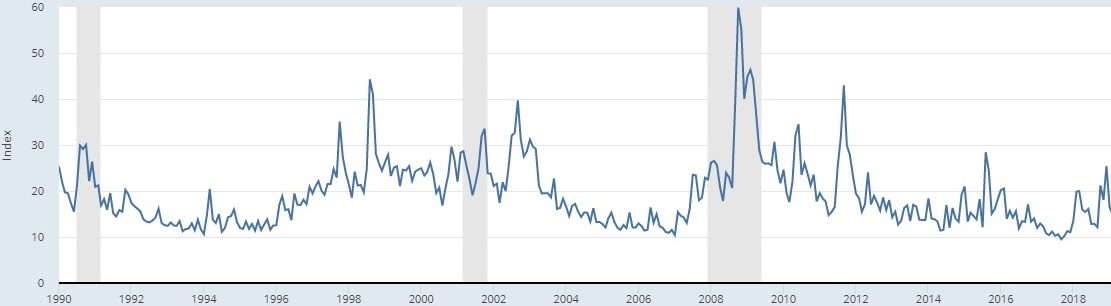
\includegraphics[width=1\textwidth]{vix_90.jpg}

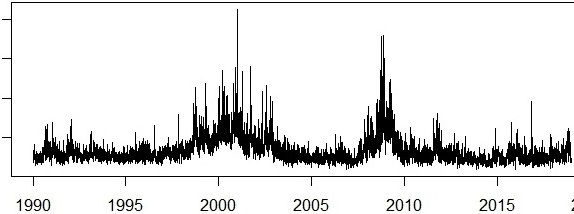
\includegraphics[width=1\textwidth]{ts_cid_90_01.jpg}
\end{frame}



\end{document}

